% ----------------------------------------------------------------------
%
%        Vorlage für Abschlussarbeiten am Lehrstuhl Informatik VII
%
%                   http://ls7-www.cs.uni-dortmund.de
%
%   Für Fragen und Anregungen zur Vorlage: info@ls7.cs.uni-dortmund.de
%
%   Stand: 27.05.2012
%
% ----------------------------------------------------------------------

\RequirePackage{ifthen}
%
% Arbeitsbezeichnung: Bachelor-Arbeit, Master-Arbeit, Diplomarbeit
%
\newcommand \Arbeitsbezeichnung{Bachelor-Arbeit}
\newcommand \Autor{Vorname Nachname}
\newcommand \Arbeitstitel{Dieses ist der Titel der Bachelorarbeit}
\newcommand \Erstgutachter{Prof.~Dr.~Vorname~Nachname}
\newcommand \Zweitgutachter{Dipl.-Inform.~Vorname~Nachname}
\newcommand \ErstLehrstuhl{Lehrstuhl Informatik VII}
\newcommand \ErstLehrstuhltitel{Graphische Systeme}

% -----------------------------------------------------------------------------------------
% Option: Zweiter Lehrstuhl
\newboolean{boolkeinZweitLS}
\setboolean{boolkeinZweitLS}{true} % Zuweisung auf ''false'' sofern zweiter Lehrstuhl beteiligt
\ifthenelse{\boolean{boolkeinZweitLS}}{
\newcommand \ZweitLehrstuhl{}
\newcommand \ZweitLehrstuhltitel{}
}{
\newcommand \ZweitLehrstuhl{Lehrstuhl Informatik XII}
\newcommand \ZweitLehrstuhltitel{Eingebettete Systeme}
}

\RequirePackage{ifpdf} \ifpdf
  \pdfoutput=1
  \pdftrue
  \message{pdfLaTeX}
  \documentclass[pdftex,12pt,a4paper,twoside,ngerman]{scrbook}
  \usepackage{float}
  \usepackage[pdftex]{thumbpdf}
  \usepackage[pdftex]{graphicx}
  \usepackage[pdftex]{hyperref}
  \usepackage{pdfpages}
  \pdfoutput=1
  \pdfcompresslevel=9
  \DeclareGraphicsExtensions{.pdf,.jpg,.png}
\else
  \pdffalse
  \message{LaTeX}
  \documentclass[dvips,12pt,a4paper,twoside,ngerman]{scrbook}
  \usepackage{float}
  \usepackage{graphicx}
  \usepackage{epsf}
  \usepackage[dvips]{hyperref}
  \DeclareGraphicsExtensions{.eps}
\fi


% Informationen fuer pdf-File festlegen
\hypersetup
{
    pdfauthor = {\Autor},
    pdftitle = {\Arbeitstitel},
    pdfsubject = {\Arbeitsbezeichnung, TU Dortmund, Fakult{\"a}t f{\"u}r Informatik},
    pdfproducer = {LaTeX},
    pdfview = FitV,
    pdfstartview = FitV,
    pdfhighlight = /I,
    pdfborder = 0 0 0,
    colorlinks = false,
    bookmarksopen,
    bookmarksopenlevel = 1,
    bookmarksnumbered = false,
    plainpages = false
}%


% Seitenformat anpassen
\usepackage[a4paper,left=3.5cm,right=2.5cm,bottom=3.5cm,top=3cm]{geometry}
\setlength{\headheight}{15pt}
% -------------------------------------------------------------------
% Grafikpakete einbinden
\usepackage{amsmath,amssymb}
\usepackage{flafter}
\usepackage{subfigure}

% -------------------------------------------------------------------
\usepackage{ifthen}

% -------------------------------------------------------------------
\usepackage[absolute,overlay]{textpos}
\setlength{\TPHorizModule}{1mm}
\setlength{\TPVertModule}{\TPHorizModule}
\textblockorigin{0mm}{0mm}
\usepackage{fix-cm}
\usepackage{setspace}
\usepackage{scrhack}
% -------------------------------------------------------------------
% Korrekte Darstellung der Umlaute
\usepackage[german,ngerman]{babel}
\usepackage[utf8]{inputenc}
\usepackage[T1]{fontenc}
\usepackage{ae,aecompl}


% -------------------------------------------------------------------
% Bibtex deutsch
\usepackage[numbers,sort]{natbib}


% -------------------------------------------------------------------
% Anführungszeichen
\usepackage[babel,german=quotes]{csquotes}


% -------------------------------------------------------------------
% URLs
\usepackage{url}

% -------------------------------------------------------------------
% Caption anpassen
\usepackage[margin=0pt,font=small,labelfont=bf]{caption}

% -------------------------------------------------------------------
% Erweitere Tabellen
\usepackage{booktabs}

% -------------------------------------------------------------------
% Eurosymbol
\usepackage{eurosym}

% -------------------------------------------------------------------
% Zeilenabstand einstellen
\renewcommand{\baselinestretch}{1.25}
% Floating-Umgebungen anpassen
\renewcommand{\topfraction}{0.9}
\renewcommand{\bottomfraction}{0.8}

% -------------------------------------------------------------------
% Keine einzelnen Zeilen beim Anfang eines Abschnitts (Schusterjungen)
%\clubpenalty = 10000
% Keine einzelnen Zeilen am Ende eines Abschnitts (Hurenkinder)
%\widowpenalty = 10000 \displaywidowpenalty = 10000

\parindent=0cm


% -------------------------------------------------------------------
% Kopfzeile hinzufuegen
\usepackage{fancyhdr}
\usepackage{extramarks}

\pagestyle{fancy}
\renewcommand{\chaptermark}[1]{\markboth{#1}{}}
\renewcommand{\sectionmark}[1]{\markright{#1}{}}

\fancyhf{}
\fancyhead[LE,RO]{\thepage}
\fancyhead[RE]{\textit{\nouppercase{\leftmark}}}
\fancyhead[LO]{\textit{\nouppercase{\rightmark}}}

\fancypagestyle{plain}{ %
\fancyhf{} % remove everything
\renewcommand{\headrulewidth}{0pt} % remove lines as well
\renewcommand{\footrulewidth}{0pt}} \pagestyle{headings}



% -------------------------------------------------------------------
% Eigene Farben definieren
\usepackage{color}
\definecolor{TUGreen}{rgb}{0.517,0.721,0.094}
\definecolor{TUOrange}{rgb}{1.0,0.7176,0.0}
\definecolor{BrightGray}{gray}{0.9}
\definecolor{DarkGray}{gray}{0.2}
\definecolor{white}{rgb}{1,1,1}
\definecolor{black}{rgb}{0,0,0}
\definecolor{red}{rgb}{1,0,0}




% -------------------------------------------------------------------
% Programm-Listings einbinden und formatieren
\usepackage{listings}

\lstdefinestyle{C++}
{
language=C++,
backgroundcolor=\color{BrightGray},
keywordstyle=\tt\bfseries,  %\color{TUGreen}\bfseries,
commentstyle=\color{DarkGray},
stringstyle=\color{red},
showstringspaces=false,
basicstyle=\small\color{black},
numbers=left,
captionpos=b,
tabsize=4,
breaklines=true
}


% -------------------------------------------------------------------
% Algorithmen
\usepackage[plain,chapter]{algorithm}
\usepackage{algorithmic}

\usepackage{enumerate}

% -------------------------------------------------------------------
% Algorithmen anpassen
\renewcommand{\algorithmicrequire}{\textit{Eingabe:}}
\renewcommand{\algorithmicensure}{\textit{Ausgabe:}}
\floatname{algorithm}{Algorithmus}
\renewcommand{\listalgorithmname}{Algorithmenverzeichnis}
\renewcommand{\algorithmiccomment}[1]{\color{grau}{// #1}}


% -------------------------------------------------------------------
% -------------------------------------------------------------------
% -------------------------------------------------------------------
\begin{document}
\pagenumbering{alpha}

%========================================================================================
% TU Dortmund, Informatik Lehrstuhl VII
%========================================================================================

\begin{titlepage}

\begin{textblock}{150}(30.5,10.75)%
\raggedright

\includegraphics[width=83.25mm]{bilder/tud_logo_cmyk.pdf}%
\end{textblock}

\begin{textblock}{150}(21.2,41.6)%
\raggedright\sf%\Huge
{\color{red}\rule{5mm}{5mm}}
\end{textblock}

\begin{textblock}{150}(30.4,40.32)%
\raggedright

\includegraphics[width=90mm]{bilder/fi_text.pdf}
\end{textblock}

\begin{textblock}{89}(35.0,62.75)%
\begin{minipage}{80mm}
	\vfill
	\begin{center}
	\fontsize{24pt}{24pt} \sf
	\Arbeitsbezeichnung
	
	\vspace{1cm}
	\begin{onehalfspace}
    \fontsize{18pt}{18pt}
    \sf \Arbeitstitel
    \end{onehalfspace}
	
	\vspace{12mm}
\begin{onehalfspace}
	{\fontsize{14pt}{14pt}\sf \Autor

	\today}
 \end{onehalfspace}
	\end{center}
	\vfill
\end{minipage}\end{textblock}

\begin{textblock}{150}(44.25,208)%
\begin{minipage}{120mm}
	\large
	\raggedright
	\sf
    {\fontsize{14pt}{14pt}
	\textbf{Gutachter:}\\
	\Erstgutachter\\
	\Zweitgutachter\\}
\end{minipage}
\end{textblock}



\begin{textblock}{150}(44.25,242.0)%
\ifthenelse{\boolean{boolkeinZweitLS}}{
%
\begin{minipage}{120mm}
	\fontsize{11.75pt}{11.75pt}\selectfont
	\raggedright
	\sf
	\textcolor{TUGreen}{\ErstLehrstuhl}\\
	\textcolor{TUGreen}{\ErstLehrstuhltitel}\\
    \textcolor{TUGreen}{TU Dortmund}
\end{minipage}
%
}{
%
\begin{tabular*}{\textwidth}[t]{c c}%
  \begin{minipage}[t]{70mm}
    \raggedright
	\sf
    \textcolor{TUGreen}{\ErstLehrstuhl}\\
    \textcolor{TUGreen}{(\ErstLehrstuhltitel)}\\
    \textcolor{TUGreen}{TU Dortmund}
    \end{minipage}
    \hspace*{0.5cm}
    \begin{minipage}[t]{70mm}
    \raggedright
	\sf    
    \textcolor{TUOrange}{\ZweitLehrstuhl}\\
    \textcolor{TUOrange}{(\ZweitLehrstuhltitel)}\\
    \textcolor{TUOrange}{TU Dortmund}
  \end{minipage}
\end{tabular*}
%
}
%
\end{textblock}



\vspace*{20cm}



\end{titlepage}


\pagestyle{empty} \cleardoublepage

\pagenumbering{roman} \tableofcontents

\cleardoublepage \pagestyle{headings}

\pagenumbering{arabic}

% -------------------------------------------------------------------

\pagestyle{empty}
%========================================================================================
% TU Dortmund, Informatik Lehrstuhl VII
%========================================================================================

\chapter*{Mathematische Notation} \label{Notation}
\addcontentsline{toc}{chapter}{Mathematische Notation}

\newcommand{\tabdummy}{\midrule[0pt]}

\begin{tabular}{p{0.25\textwidth}p{0.65\textwidth}}
  \textbf{Notation} & \textbf{Bedeutung} \\ \toprule[1pt]
   $\mathbb{N}$ & Menge der natürlichen Zahlen ${1, 2, 3, \ldots}$ \\ \tabdummy
   $\mathbb{R}$ & Menge der reellen Zahlen \\ \tabdummy
   $\mathbb{R}^d$ & $d$-dimensionaler Raum\\ \tabdummy
   $\mathcal{M} = \{m_1,\ldots,m_N\}$ & Menge $\mathcal{M}$ von $N$ Elementen $m_i$ \\ \tabdummy
   $G=(V,E)$ & Graph $G$ mit Knotenmenge $V$ und Kantenmenge $E$ \\ \tabdummy
   $\mathbf{p}$ & Vektor\\ \tabdummy
   $\mathbf{p}_i$ & $i$-tes Element eines Vektors \\ \tabdummy
   $\mathbf{v}^{(j)}_i$ & $i$-tes Element des $j$-ten Vektors \\ \tabdummy
   $\mathbf{A}$ & Matrix
\end{tabular}

\cleardoublepage

\pagestyle{fancy}

%========================================================================================
% TU Dortmund, Informatik Lehrstuhl VII
%========================================================================================

\chapter{Einleitung}
\label{Einleitung}

\section{Motivation und Hintergrund}
\label{Motivation_und_Hintergrund}
%
Literatur \cite{Abramowski:1991} oder \cite{Abramowski:1991, Muller:2011} und Verweis auf Kapitel
\ref{Kapitel 2} ab Seite \pageref{Kapitel 2}.



\section{Aufbau der Arbeit}
\label{Aufbau_der_Arbeit}
%
Er hörte \enquote{leise Schritte} hinter sich. Das bedeutete
nichts Gutes. Wer würde ihm schon folgen, spät in der Nacht und
dazu noch in dieser engen Gasse mitten im übel beleumundeten
Hafenviertel\footnote{Wer würde ihm schon folgen.}? Gerade jetzt, wo er das Ding seines Lebens gedreht
hatte und mit der Beute verschwinden wollte! Hatte einer seiner
zahllosen Kollegen dieselbe Idee gehabt, ihn beobachtet und
abgewartet, um ihn nun um die Früchte seiner Arbeit zu
erleichtern? Oder gehörten die Schritte hinter ihm zu einem der
unzähligen Gesetzeshüter dieser Stadt, und die stählerne Acht um
seine Handgelenke würde gleich zuschnappen? Er konnte die
Aufforderung stehen zu bleiben
schon hören.

Gehetzt sah er sich um. Plötzlich erblickte er den schmalen
Durchgang. Blitzartig drehte er sich nach rechts und verschwand
zwischen den beiden Gebäuden. Beinahe wäre er dabei über den
umgestürzten Mülleimer gefallen, der mitten im Weg lag. Er
versuchte, sich in der Dunkelheit seinen Weg zu ertasten und
erstarrte: Anscheinend gab es keinen anderen Ausweg aus diesem
kleinen Hof als den Durchgang, durch den er gekommen war. Die
Schritte wurden lauter und lauter, er sah eine dunkle Gestalt um
die Ecke biegen. Fieberhaft irrten seine Augen durch die
nächtliche Dunkelheit und suchten einen Ausweg. War jetzt wirklich
alles vorbei, waren alle Mühe und alle Vorbereitungen umsonst?

Er presste sich ganz eng an die Wand hinter ihm und hoffte, der
Verfolger würde ihn übersehen, als plötzlich neben ihm mit kaum
wahrnehmbarem Quietschen eine Tür im nächtlichen Wind hin und her
schwang. Könnte dieses der flehentlich herbeigesehnte Ausweg aus
seinem Dilemma sein? Langsam bewegte er sich auf die offene Tür
zu, immer dicht an die Mauer gepresst. Würde diese Tür seine
Rettung werden? Er hörte leise Schritte hinter sich. Das bedeutete
nichts Gutes. Wer würde ihm schon folgen, spät in der Nacht und
dazu noch in dieser engen Gasse mitten im übel beleumundeten
Hafenviertel? Gerade jetzt, wo er das Ding seines Lebens gedreht
hatte und mit der Beute verschwinden wollte! Hatte einer seiner
zahllosen Kollegen dieselbe Idee gehabt, ihn beobachtet und
abgewartet, um ihn nun um die Früchte seiner Arbeit zu
erleichtern? Oder gehörten die Schritte hinter ihm zu einem der
unzähligen Gesetzeshüter dieser Stadt, und die stählerne Acht um
seine Handgelenke würde gleich zuschnappen? Er konnte die
Aufforderung stehen zu bleiben schon hören. Gehetzt sah er sich
um. Plötzlich erblickte er den schmalen Durchgang. Blitzartig
drehte er sich nach rechts und verschwand zwischen den beiden
Gebäuden.

Er hörte \enquote{leise Schritte} hinter sich. Das bedeutete
nichts Gutes. Wer würde ihm schon folgen, spät in der Nacht und
dazu noch in dieser engen Gasse mitten im übel beleumundeten
Hafenviertel? Gerade jetzt, wo er das Ding seines Lebens gedreht
hatte und mit der Beute verschwinden wollte! Hatte einer seiner
zahllosen Kollegen dieselbe Idee gehabt, ihn beobachtet und
abgewartet, um ihn nun um die Früchte seiner Arbeit zu
erleichtern? Oder gehörten die Schritte hinter ihm zu einem der
unzähligen Gesetzeshüter dieser Stadt, und die stählerne Acht um
seine Handgelenke würde gleich zuschnappen? Er konnte die
Aufforderung stehen zu bleiben
schon hören.

Gehetzt sah er sich um. Plötzlich erblickte er den schmalen
Durchgang. Blitzartig drehte er sich nach rechts und verschwand
zwischen den beiden Gebäuden. Beinahe wäre er dabei über den
umgestürzten Mülleimer gefallen, der mitten im Weg lag. Er
versuchte, sich in der Dunkelheit seinen Weg zu ertasten und
erstarrte: Anscheinend gab es keinen anderen Ausweg aus diesem
kleinen Hof als den Durchgang, durch den er gekommen war. Die
Schritte wurden lauter und lauter, er sah eine dunkle Gestalt um
die Ecke biegen. Fieberhaft irrten seine Augen durch die
nächtliche Dunkelheit und suchten einen Ausweg. War jetzt wirklich
alles vorbei, waren alle Mühe und alle Vorbereitungen umsonst?

Er presste sich ganz eng an die Wand hinter ihm und hoffte, der
Verfolger würde ihn übersehen, als plötzlich neben ihm mit kaum
wahrnehmbarem Quietschen eine Tür im nächtlichen Wind hin und her
schwang. Könnte dieses der flehentlich herbeigesehnte Ausweg aus
seinem Dilemma sein? Langsam bewegte er sich auf die offene Tür
zu, immer dicht an die Mauer gepresst. Würde diese Tür seine
Rettung werden? Er hörte leise Schritte hinter sich. Das bedeutete
nichts Gutes. Wer würde ihm schon folgen, spät in der Nacht und
dazu noch in dieser engen Gasse mitten im übel beleumundeten
Hafenviertel? Gerade jetzt, wo er das Ding seines Lebens gedreht
hatte und mit der Beute verschwinden wollte! Hatte einer seiner
zahllosen Kollegen dieselbe Idee gehabt, ihn beobachtet und
abgewartet, um ihn nun um die Früchte seiner Arbeit zu
erleichtern? Oder gehörten die Schritte hinter ihm zu einem der
unzähligen Gesetzeshüter dieser Stadt, und die stählerne Acht um
seine Handgelenke würde gleich zuschnappen? Er konnte die
Aufforderung stehen zu bleiben schon hören. Gehetzt sah er sich
um. Plötzlich erblickte er den schmalen Durchgang. Blitzartig
drehte er sich nach rechts und verschwand zwischen den beiden
Gebäuden.


\cleardoublepage
%========================================================================================
% TU Dortmund, Informatik Lehrstuhl VII
%========================================================================================

\chapter{Berechnungen}



\section{Bestimmung der Bewegung}
\subsection{BoundigBox Methode}
\subsection{BoundingSphere Methode}
\label{Kapitel_2_-_Unterkapitel_1}

\section{Bestimmung der Pose}
\subsection{BoundingBox Methode}
\subsection{Proportionalitäts Methode}

\section{Bestimmung der Blickrichtung}
\subsection{Rückprojektions Methode}
\subsection{Historgamm Methode}



%


\cleardoublepage
%========================================================================================
% TU Dortmund, Informatik Lehrstuhl VII
%========================================================================================

\chapter{Das Kapitel 3}
\label{Kapitel 3}
%
Gehetzt sah er sich um. Plötzlich erblickte er den schmalen
Durchgang. Blitzartig drehte er sich nach rechts und verschwand
zwischen den beiden Gebäuden. Beinahe wäre er dabei über den
umgestürzten Mülleimer gefallen, der mitten im Weg lag. Er
versuchte, sich in der Dunkelheit seinen Weg zu ertasten und
erstarrte: Anscheinend gab es keinen anderen Ausweg aus diesem
kleinen Hof als den Durchgang, durch den er gekommen war.

\section{Kapitel 3 - Unterkapitel 1}
\label{Kapitel_3_-_Unterkapitel_1}
%
    \begin{algorithm}[t]
    \centering
    \caption[Ein Algorithmus]{Algorithmus} \label{algo_1}
    \begin{algorithmic}
    \REQUIRE Wert $x :=3$
    \ENSURE Wert für $y$
    \STATE $z = 2$
    \WHILE{$(z < 10)$}
    \STATE $x = x + z$
    \FOR{$(1 \leq a \leq z-1)$}
    \STATE $z = z + 1$
    \ENDFOR
    \ENDWHILE
    \end{algorithmic}
    \end{algorithm}


Er hörte \enquote{leise Schritte} hinter sich. Das bedeutete
nichts Gutes. Wer würde ihm schon folgen, spät in der Nacht und
dazu noch in dieser engen Gasse mitten im übel beleumundeten
Hafenviertel? Gerade jetzt, wo er das Ding seines Lebens gedreht
hatte und mit der Beute verschwinden wollte! Hatte einer seiner
zahllosen Kollegen dieselbe Idee gehabt, ihn beobachtet und
abgewartet, um ihn nun um die Früchte seiner Arbeit zu
erleichtern? Oder gehörten die Schritte hinter ihm zu einem der
unzähligen Gesetzeshüter dieser Stadt, und die stählerne Acht um
seine Handgelenke würde gleich zuschnappen? Er konnte die
Aufforderung stehen zu bleiben
schon hören.

Gehetzt sah er sich um. Plötzlich erblickte er den schmalen
Durchgang. Blitzartig drehte er sich nach rechts und verschwand
zwischen den beiden Gebäuden. Beinahe wäre er dabei über den
umgestürzten Mülleimer gefallen, der mitten im Weg lag. Er
versuchte, sich in der Dunkelheit seinen Weg zu ertasten und
erstarrte: Anscheinend gab es keinen anderen Ausweg aus diesem
kleinen Hof als den Durchgang, durch den er gekommen war. Die
Schritte wurden lauter und lauter, er sah eine dunkle Gestalt um
die Ecke biegen. Fieberhaft irrten seine Augen durch die
nächtliche Dunkelheit und suchten einen Ausweg. War jetzt wirklich
alles vorbei, waren alle Mühe und alle Vorbereitungen umsonst?

Er presste sich ganz eng an die Wand hinter ihm und hoffte, der
Verfolger würde ihn übersehen, als plötzlich neben ihm mit kaum
wahrnehmbarem Quietschen eine Tür im nächtlichen Wind hin und her
schwang. Könnte dieses der flehentlich herbeigesehnte Ausweg aus
seinem Dilemma sein? Langsam bewegte er sich auf die offene Tür
zu, immer dicht an die Mauer gepresst. Würde diese Tür seine
Rettung werden? Er hörte leise Schritte hinter sich. Das bedeutete
nichts Gutes. Wer würde ihm schon folgen, spät in der Nacht und
dazu noch in dieser engen Gasse mitten im übel beleumundeten
Hafenviertel? Gerade jetzt, wo er das Ding seines Lebens gedreht
hatte und mit der Beute verschwinden wollte! Hatte einer seiner
zahllosen Kollegen dieselbe Idee gehabt, ihn beobachtet und
abgewartet, um ihn nun um die Früchte seiner Arbeit zu
erleichtern? Oder gehörten die Schritte hinter ihm zu einem der
unzähligen Gesetzeshüter dieser Stadt, und die stählerne Acht um
seine Handgelenke würde gleich zuschnappen? Er konnte die
Aufforderung stehen zu bleiben schon hören. Gehetzt sah er sich
um. Plötzlich erblickte er den schmalen Durchgang. Blitzartig
drehte er sich nach rechts und verschwand zwischen den beiden
Gebäuden.


\begin{lstlisting}[style=C++, caption=Beispielcode]{Name}
#include <stdio.h>
#include <stdlib.h>

int main() {

    int counter = 100;
    for(int i = 1; i < 100; i++){
        if(counter > i) printf("Hallo");
        counter--;
    }
}

return 0;
\end{lstlisting}





\section{Kapitel 3 - Unterkapitel 2}
\label{Kapitel_3_-_Unterkapitel_2}
%
\begin{table}[b]
\centering
\begin{tabular}{lrr}
\toprule
\multicolumn{2}{c}{Studium}\\ \cmidrule{1-2}
Fach & Dauer & Einkommen (\euro{})\\
\midrule
Info & 2 & 12,75 \\ \addlinespace
MST & 6 & 8,20 \\ \addlinespace
Informatik & 14 & 10,00\\
\bottomrule
\end{tabular}
\caption{Studium}
\label{table:Studium}
\end{table}
%
Er presste sich ganz eng an die Wand hinter ihm und hoffte, der
Verfolger würde ihn übersehen, als plötzlich neben ihm mit kaum
wahrnehmbarem Quietschen eine Tür im nächtlichen Wind hin und her
schwang. Könnte dieses der flehentlich herbeigesehnte Ausweg aus
seinem Dilemma sein? Langsam bewegte er sich auf die offene Tür
zu, immer dicht an die Mauer gepresst. Würde diese Tür seine
Rettung werden? Er hörte leise Schritte hinter sich. Das bedeutete
nichts Gutes. Wer würde ihm schon folgen, spät in der Nacht und
dazu noch in dieser engen Gasse mitten im übel beleumundeten
Hafenviertel? Gerade jetzt, wo er das Ding seines Lebens gedreht
hatte und mit der Beute verschwinden wollte! Hatte einer seiner
zahllosen Kollegen dieselbe Idee gehabt, ihn beobachtet und
abgewartet, um ihn nun um die Früchte seiner Arbeit zu
erleichtern? Oder gehörten die Schritte hinter ihm zu einem der
unzähligen Gesetzeshüter dieser Stadt, und die stählerne Acht um
seine Handgelenke würde gleich zuschnappen? Er konnte die
Aufforderung stehen zu bleiben schon hören. Gehetzt sah er sich
um. Plötzlich erblickte er den schmalen Durchgang. Blitzartig
drehte er sich nach rechts und verschwand zwischen den beiden
Gebäuden.

    \begin{figure}[t]
    \centering
    \subfigure[testbild2a]
          {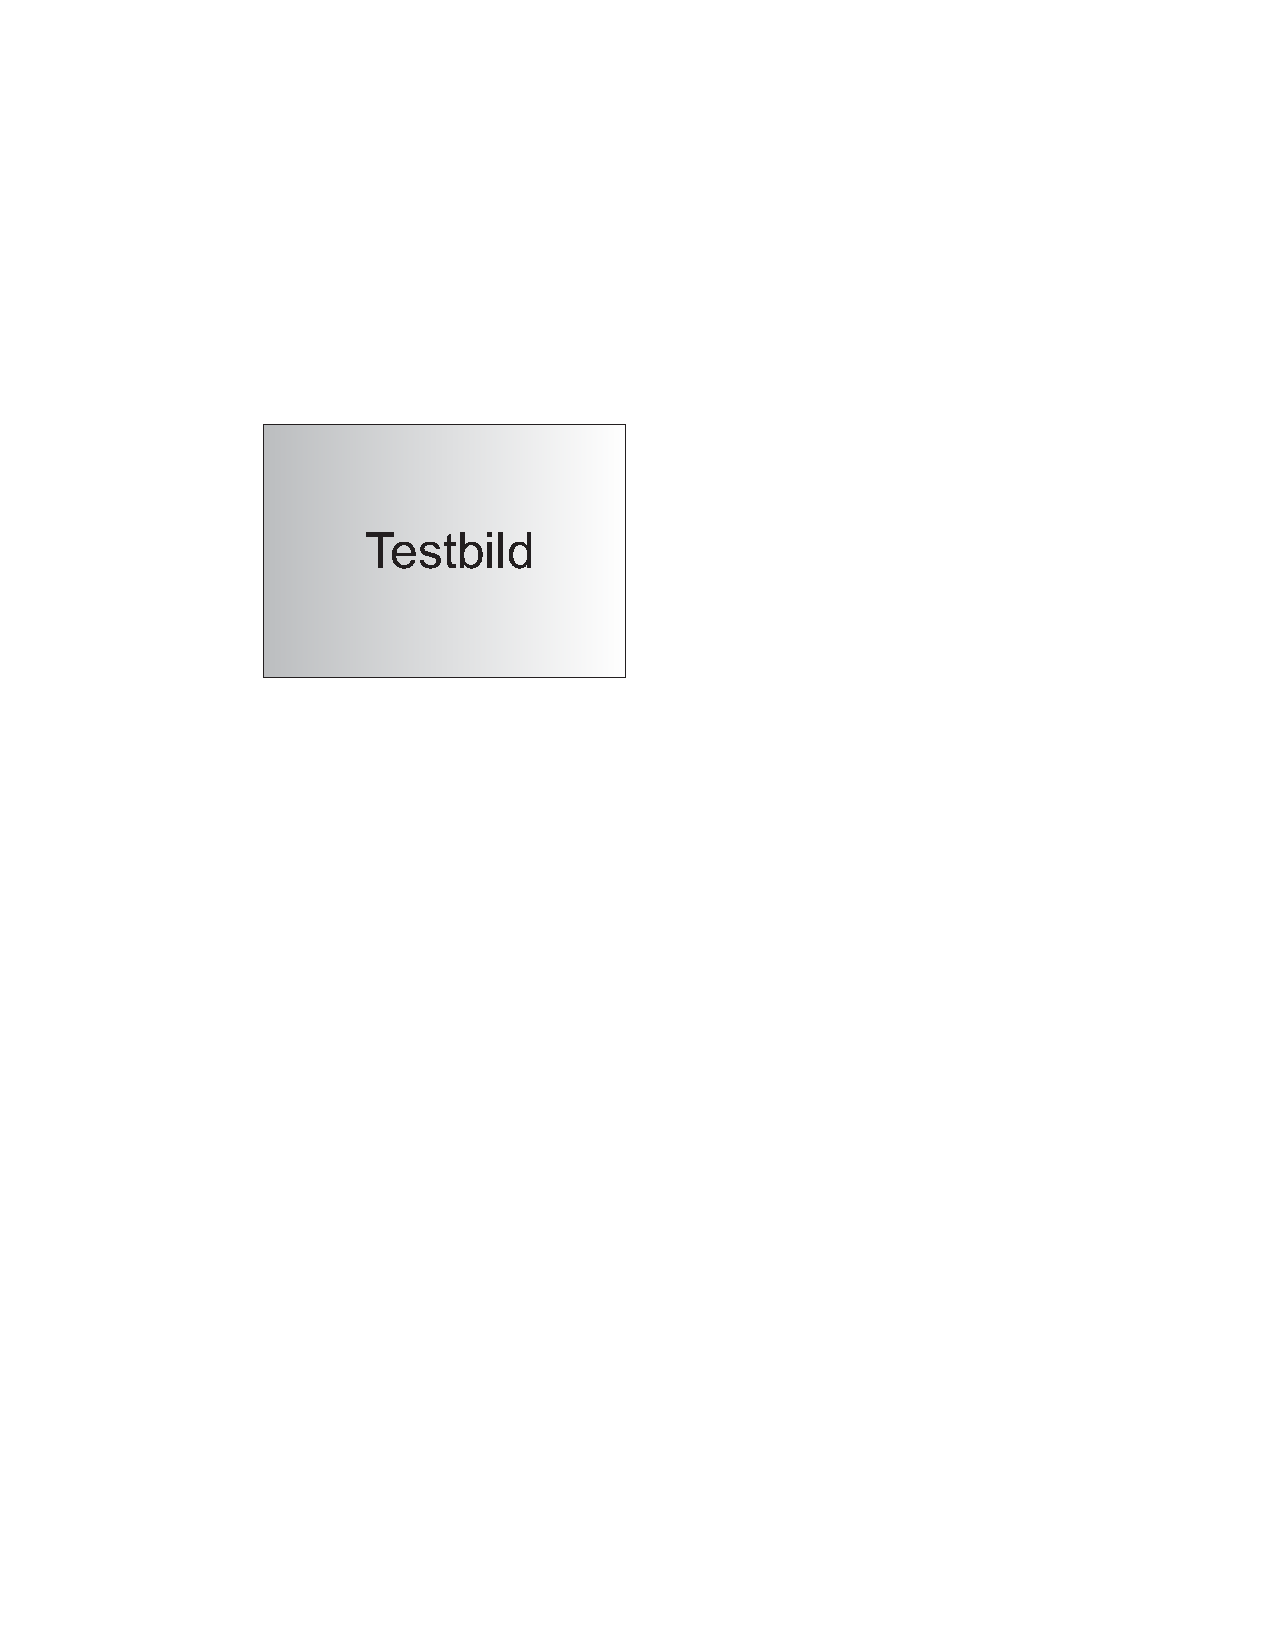
\includegraphics[scale=0.8]{bilder/testbild}\label{fig_testbild2_a}
    }
    \hspace{1.5cm}%
    \subfigure[testbild2b]
         {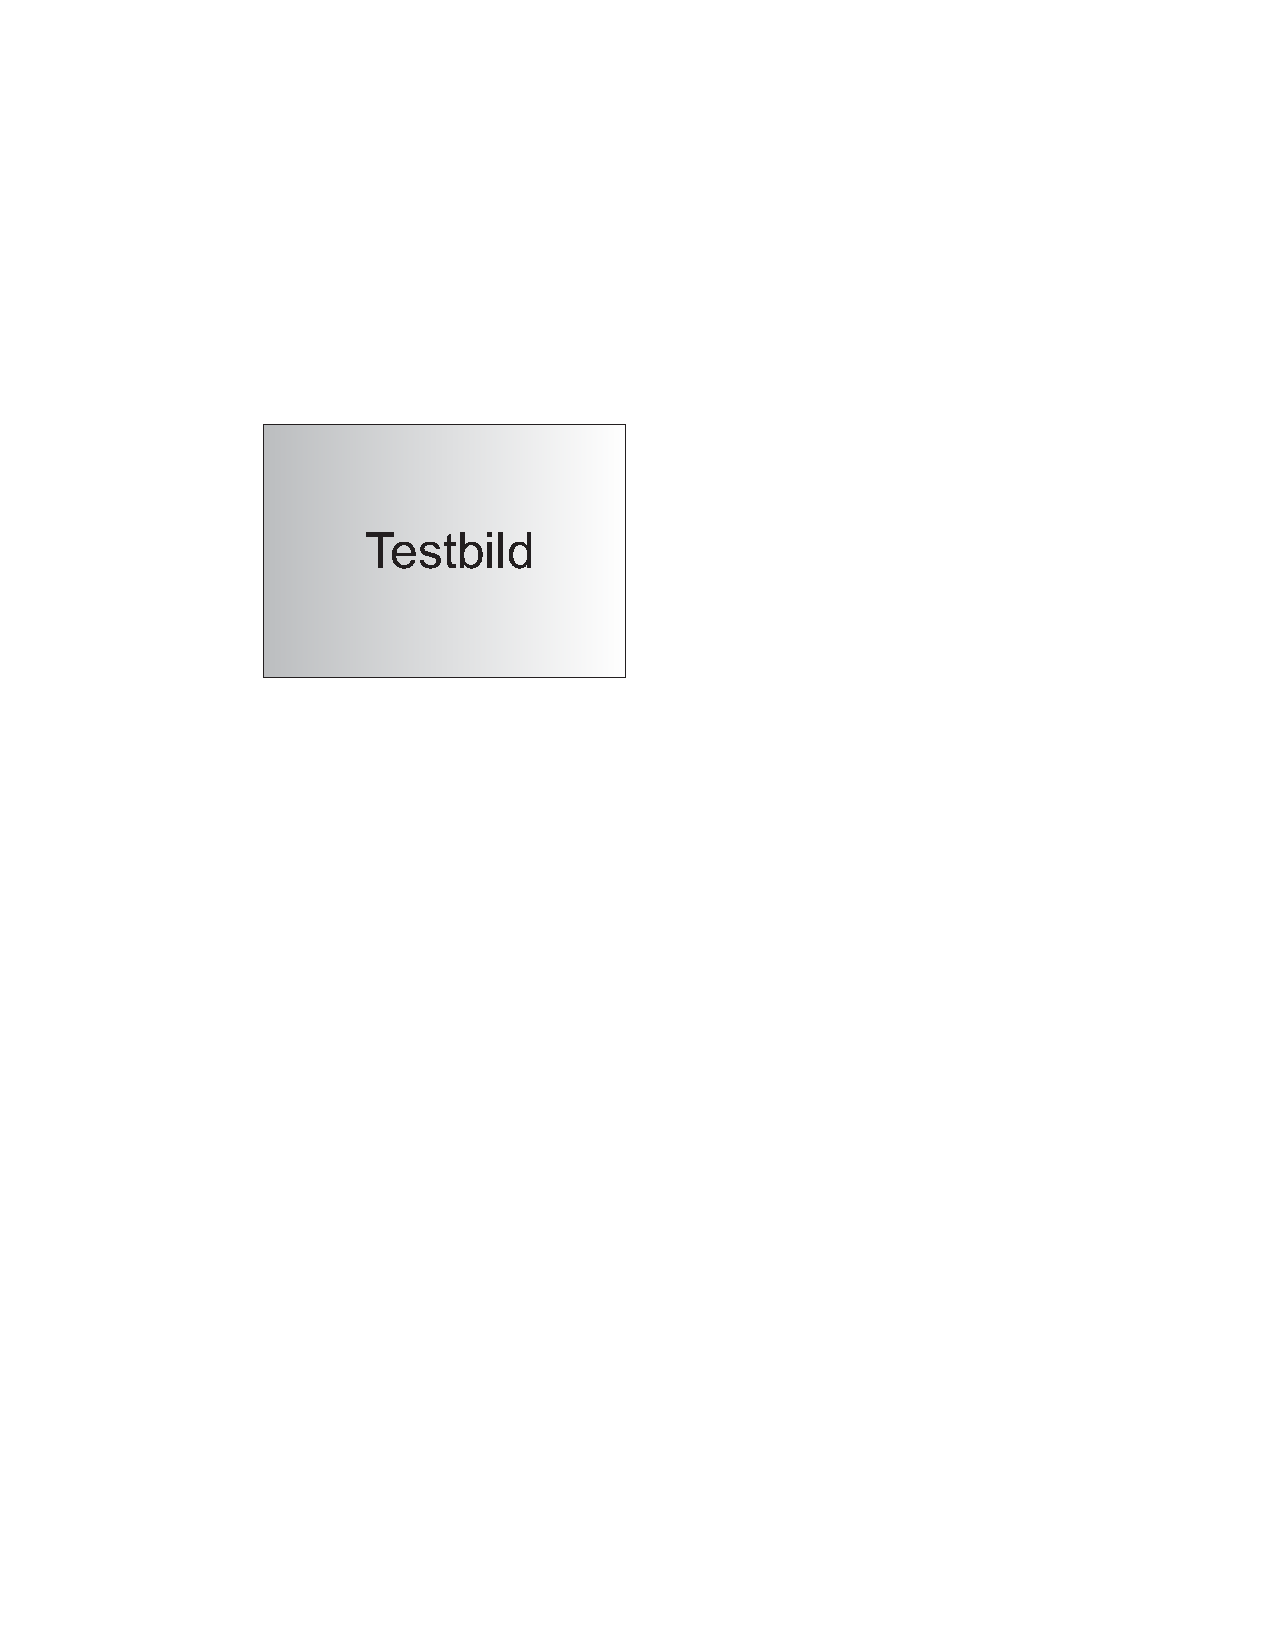
\includegraphics[scale=0.8]{bilder/testbild}\label{fig_testbild2_b}
    }\\
    \subfigure[testbild2c]
          {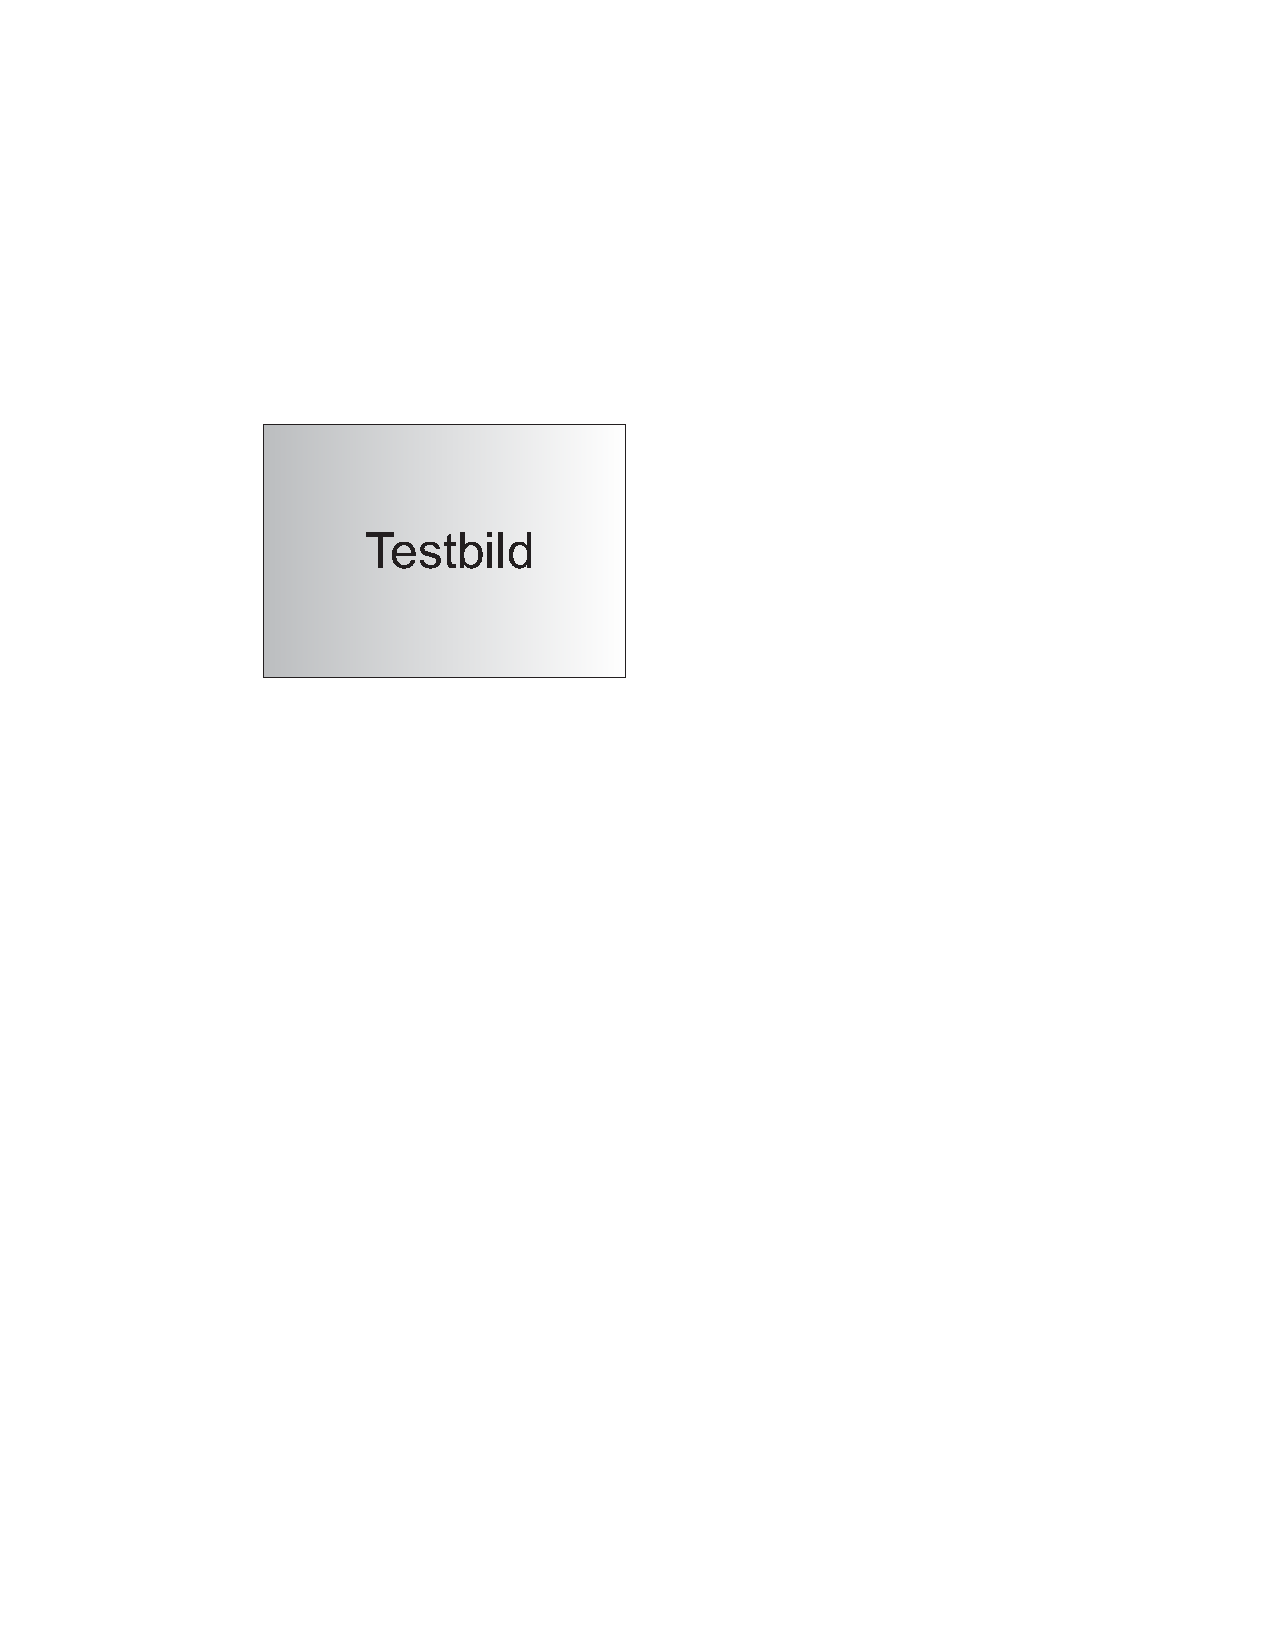
\includegraphics[scale=0.8]{bilder/testbild}\label{fig_testbild2_c}
    }
    \hspace{1.5cm}%
    \subfigure[testbild2d]
         {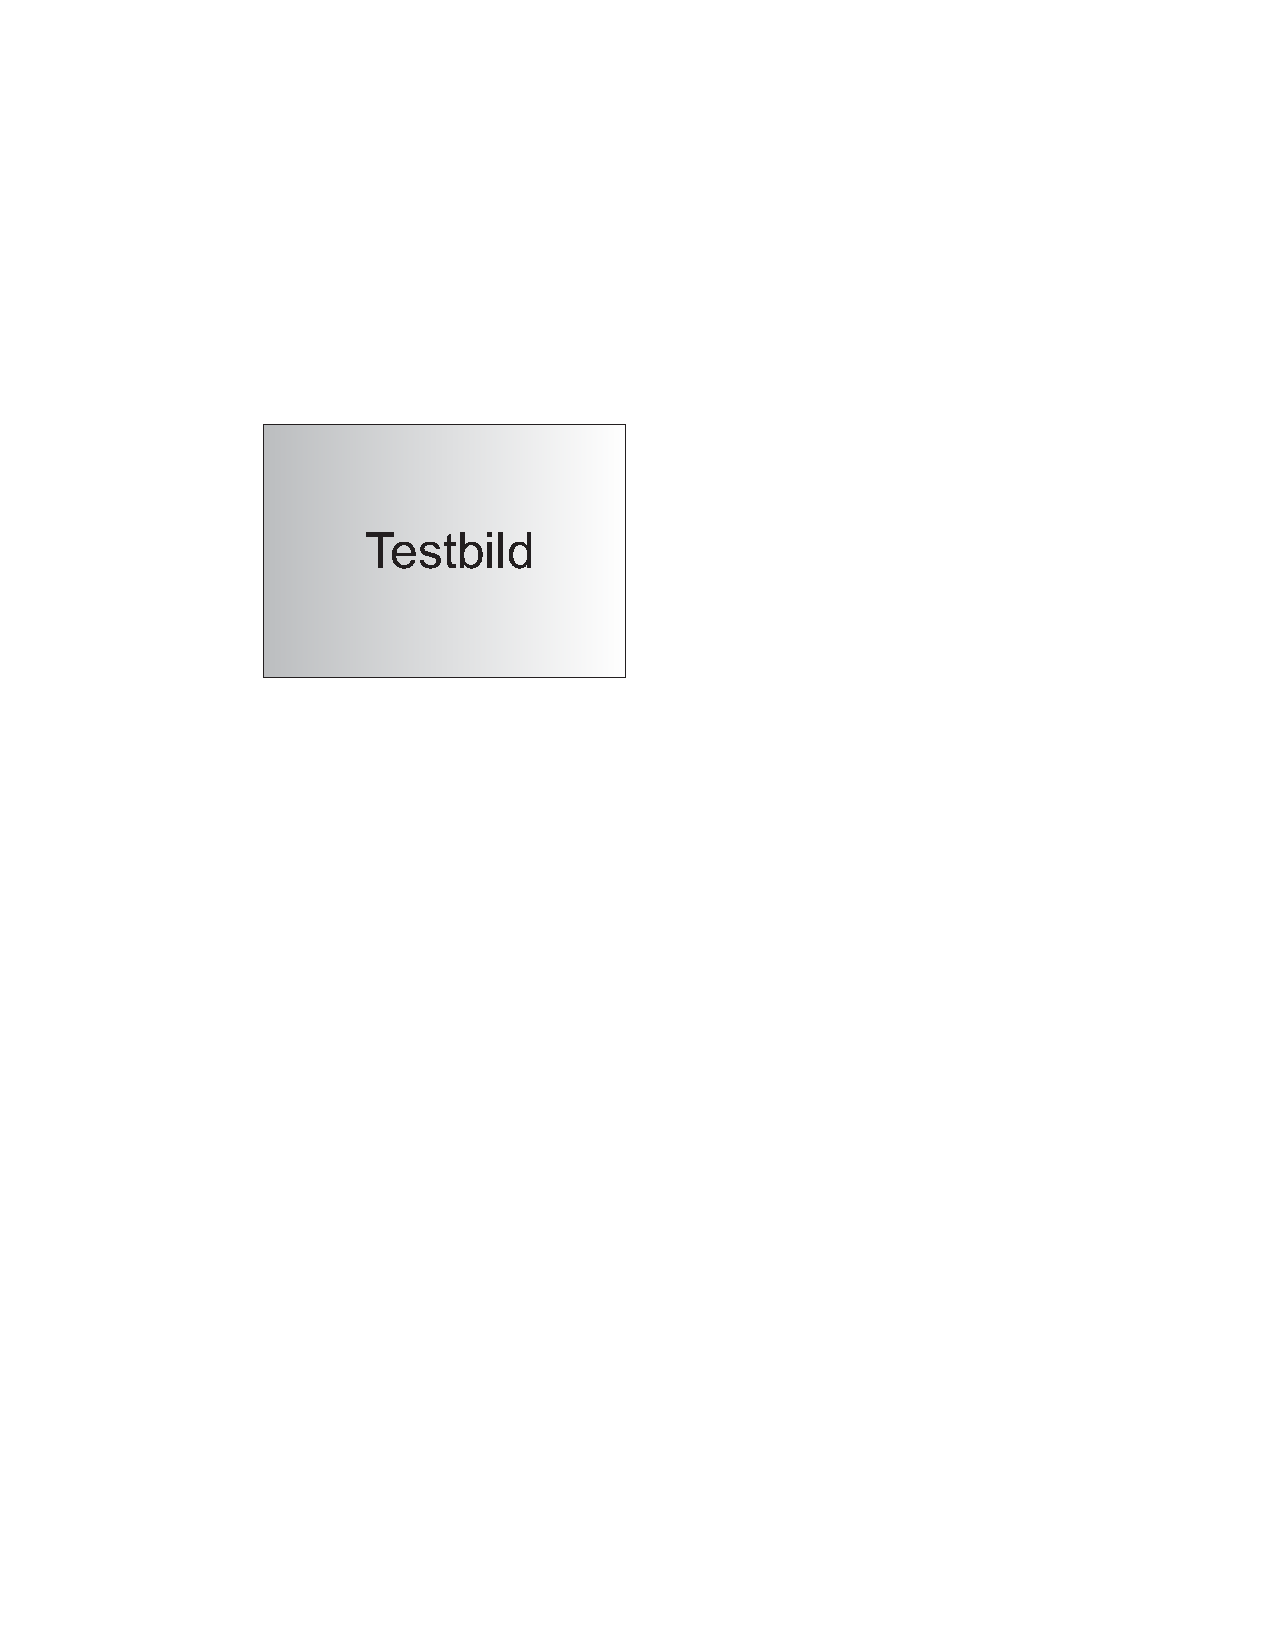
\includegraphics[scale=0.8]{bilder/testbild}\label{fig_testbild2_d}
    }\\
    \caption[Weitere Testbilder]{Weitere Testbilder}
        \label{fig_testbild2}
    \end{figure}

Er presste sich ganz eng an die Wand hinter ihm und hoffte, der
Verfolger würde ihn übersehen, als plötzlich neben ihm mit kaum
wahrnehmbarem Quietschen eine Tür im nächtlichen Wind hin und her
schwang. Könnte dieses der flehentlich herbeigesehnte Ausweg aus
seinem Dilemma sein? Langsam bewegte er sich auf die offene Tür
zu, immer dicht an die Mauer gepresst. Würde diese Tür seine
Rettung werden? Er hörte leise Schritte hinter sich. Das bedeutete
nichts Gutes. Wer würde ihm schon folgen, spät in der Nacht und
dazu noch in dieser engen Gasse mitten im übel beleumundeten
Hafenviertel? Gerade jetzt, wo er das Ding seines Lebens gedreht
hatte und mit der Beute verschwinden wollte! Hatte einer seiner
zahllosen Kollegen dieselbe Idee gehabt, ihn beobachtet und
abgewartet, um ihn nun um die Früchte seiner Arbeit zu
erleichtern? Oder gehörten die Schritte hinter ihm zu einem der
unzähligen Gesetzeshüter dieser Stadt, und die stählerne Acht um
seine Handgelenke würde gleich zuschnappen? Er konnte die
Aufforderung stehen zu bleiben schon hören. Gehetzt sah er sich
um. Plötzlich erblickte er den schmalen Durchgang. Blitzartig
drehte er sich nach rechts und verschwand zwischen den beiden
Gebäuden.

Er hörte \enquote{leise Schritte} hinter sich. Das bedeutete
nichts Gutes. Wer würde ihm schon folgen, spät in der Nacht und
dazu noch in dieser engen Gasse mitten im übel beleumundeten
Hafenviertel? Gerade jetzt, wo er das Ding seines Lebens gedreht
hatte und mit der Beute verschwinden wollte! Hatte einer seiner
zahllosen Kollegen dieselbe Idee gehabt, ihn beobachtet und
abgewartet, um ihn nun um die Früchte seiner Arbeit zu
erleichtern? Oder gehörten die Schritte hinter ihm zu einem der
unzähligen Gesetzeshüter dieser Stadt, und die stählerne Acht um
seine Handgelenke würde gleich zuschnappen? Er konnte die
Aufforderung stehen zu bleiben
schon hören.

Er hörte leise Schritte hinter sich. Das bedeutete nichts Gutes.Wer würde ihm schon folgen,
spät in der Nacht und dazu noch in dieser engen Gasse mitten im übel beleumundeten
Hafenviertel? Gerade jetzt, wo er das Ding seines Lebens gedreht hatte und mit der Beute
verschwinden wollte! Hatte einer seiner zahllosen Kollegen dieselbe Idee gehabt, ihn
beobachtet und abgewartet, um ihn nun um die Früchte seiner Arbeit zu erleichtern?
Oder gehörten die Schritte hinter ihm zu einem der unzähligen Gesetzeshüter dieser
Stadt, und die stählerne Acht um seine Handgelenke würde gleich zuschnappen? Er
konnte die Aufforderung stehen zu bleiben schon hören. Gehetzt sah er sich um. Plötzlich
erblickte er den schmalen Durchgang. Blitzartig drehte er sich nach rechts und verschwand
zwischen den beiden Gebäuden. Beinahe wäre er dabei über den umgestürzten Mülleimer
gefallen, der mitten im Weg lag. Er versuchte, sich in der Dunkelheit seinen Weg zu
ertasten und erstarrte: Anscheinend gab es keinen anderen Ausweg aus diesem kleinen
Hof als den Durchgang, durch den er gekommen war. Die Schritte wurden lauter und
lauter, er sah eine dunkle Gestalt um die Ecke biegen. Fieberhaft irrten seine Augen durch
die nächtliche Dunkelheit und suchten einen Ausweg. War jetzt wirklich alles vorbei,
waren alle Mühe und alle Vorbereitungen umsonst? Er presste sich ganz eng an die Wand
hinter ihm und hoffte, der Verfolger würde ihn übersehen, als plötzlich neben ihm mit
kaum wahrnehmbarem Quietschen eine Tür im nächtlichen Wind hin und her schwang.
Könnte dieses der flehentlich herbeigesehnte Ausweg aus seinem Dilemma sein? Langsam
bewegte er sich auf die offene Tür zu, immer dicht an die Mauer gepresst. Würde diese
Tür seine Rettung werden?

%


% -------------------------------------------------------------------

\cleardoublepage
\appendix

%========================================================================================
% TU Dortmund, Informatik Lehrstuhl VII
%========================================================================================

\chapter{Weitere Informationen}

One morning, when Gregor Samsa woke from troubled dreams, he found
himself transformed in his bed into a horrible vermin. He lay on
his armour-like back, and if he lifted his head a little he could
see his brown belly, slightly domed and divided by arches into
stiff sections. The bedding was hardly able to cover it and seemed
ready to slide off any moment. His many legs, pitifully thin
compared with the size of the rest of him, waved about helplessly
as he looked. \glqq What's happened to me?\grqq he thought. It
wasn't a dream. His room, a proper human room although a little
too small, lay peacefully between its four familiar walls. A
collection of textile samples lay spread out on the table - Samsa
was a travelling salesman - and above it there hung a picture that
he had recently cut out of an illustrated magazine and housed in a
nice, gilded frame. It showed a lady fitted out with a fur hat and
fur boa who sat upright, raising a heavy fur muff that covered the
whole of her lower arm towards the viewer. Gregor then turned to
look out the window at the dull weather. Drops of rain could be
heard hitting the pane, which made him feel quite sad.  \glqq How
about if I sleep a little bit longer and forget all this
nonsense\grqq, he thought, but that was something he was unable to
do because he was used to sleeping on his right, and in his
present state couldn't get into that position. However hard he
threw himself onto his right, he always rolled back to where he
was. He must have tried it a hundred times, shut his eyes so that
he wouldn't have to look at the floundering legs, and only stopped
when he began to feel a mild, dull pain there that he had never
felt before. \glqq Oh, God, he thought, what a strenuous career it
is that I've chosen!\grqq Travelling day in and day out. 


% -------------------------------------------------------------------

% Abbildungsverzeichnis
\listoffigures
\addcontentsline{toc}{chapter}{Abbildungsverzeichnis}
\cleardoublepage
% Algorithmenverzeichnis
\listofalgorithms
\addcontentsline{toc}{chapter}{Algorithmenverzeichnis}
\cleardoublepage
% Quellcodeverzeichnis
\renewcommand{\lstlistlistingname}{Quellcodeverzeichnis}
\lstlistoflistings
\addcontentsline{toc}{chapter}{Quellcodeverzeichnis}
\cleardoublepage

% -------------------------------------------------------------------

% Literaturverzeichnis
\addcontentsline{toc}{chapter}{Literaturverzeichnis}
\bibliographystyle{dinatls7}
\bibliography{Literatur}

% -------------------------------------------------------------------

\end{document}
